\section{Evaluation}

\subsection{Microbenchmark Evalutation}
This paper evaluate performance of different based on following microbenchmark \ref{RDMASa2a}.

\begin{figure*}[!htb]
  \centering
    \subfigure[HPC-A:MPML compared to L-a2a]{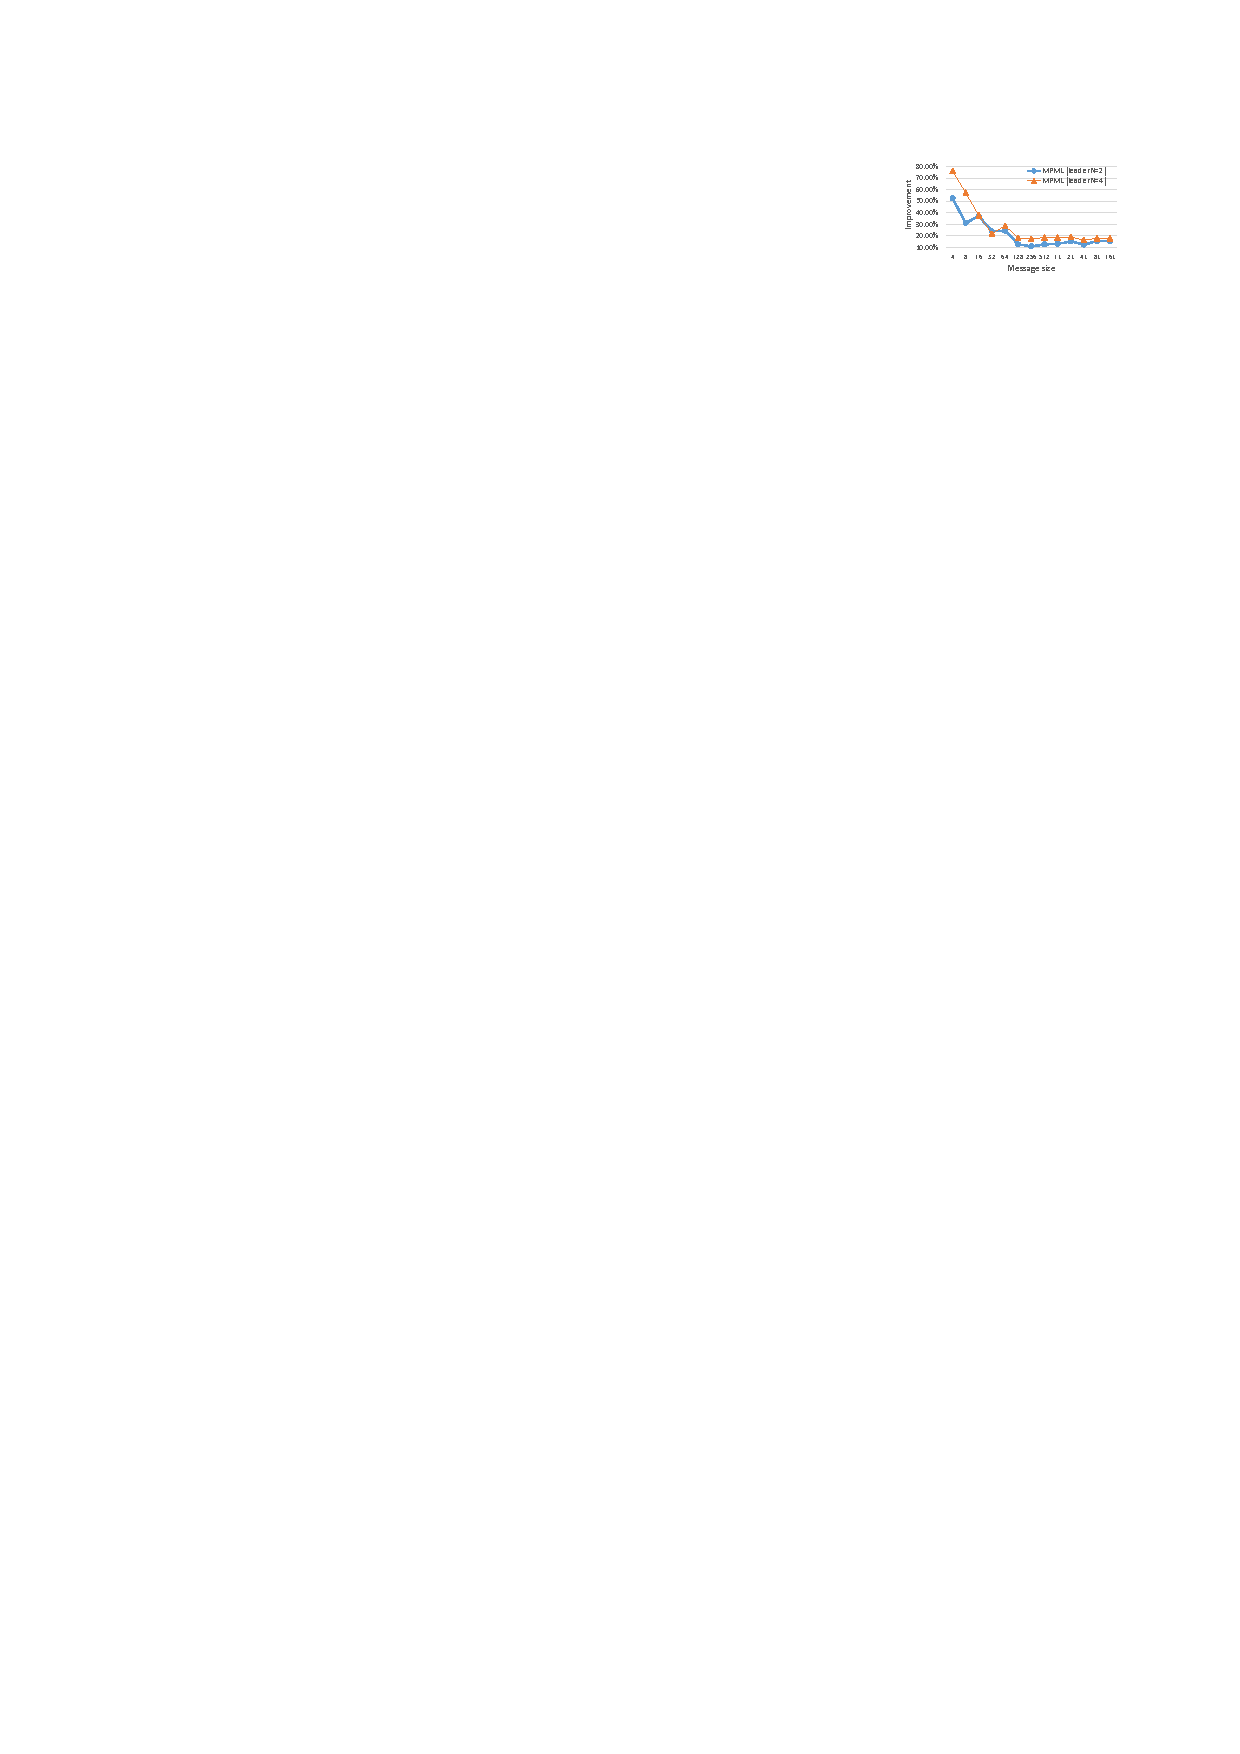
\includegraphics[width=0.45\textwidth]{./Figures/hpca/MPML.pdf}}
	\subfigure[HPC-A:NMPML compared to MPML]{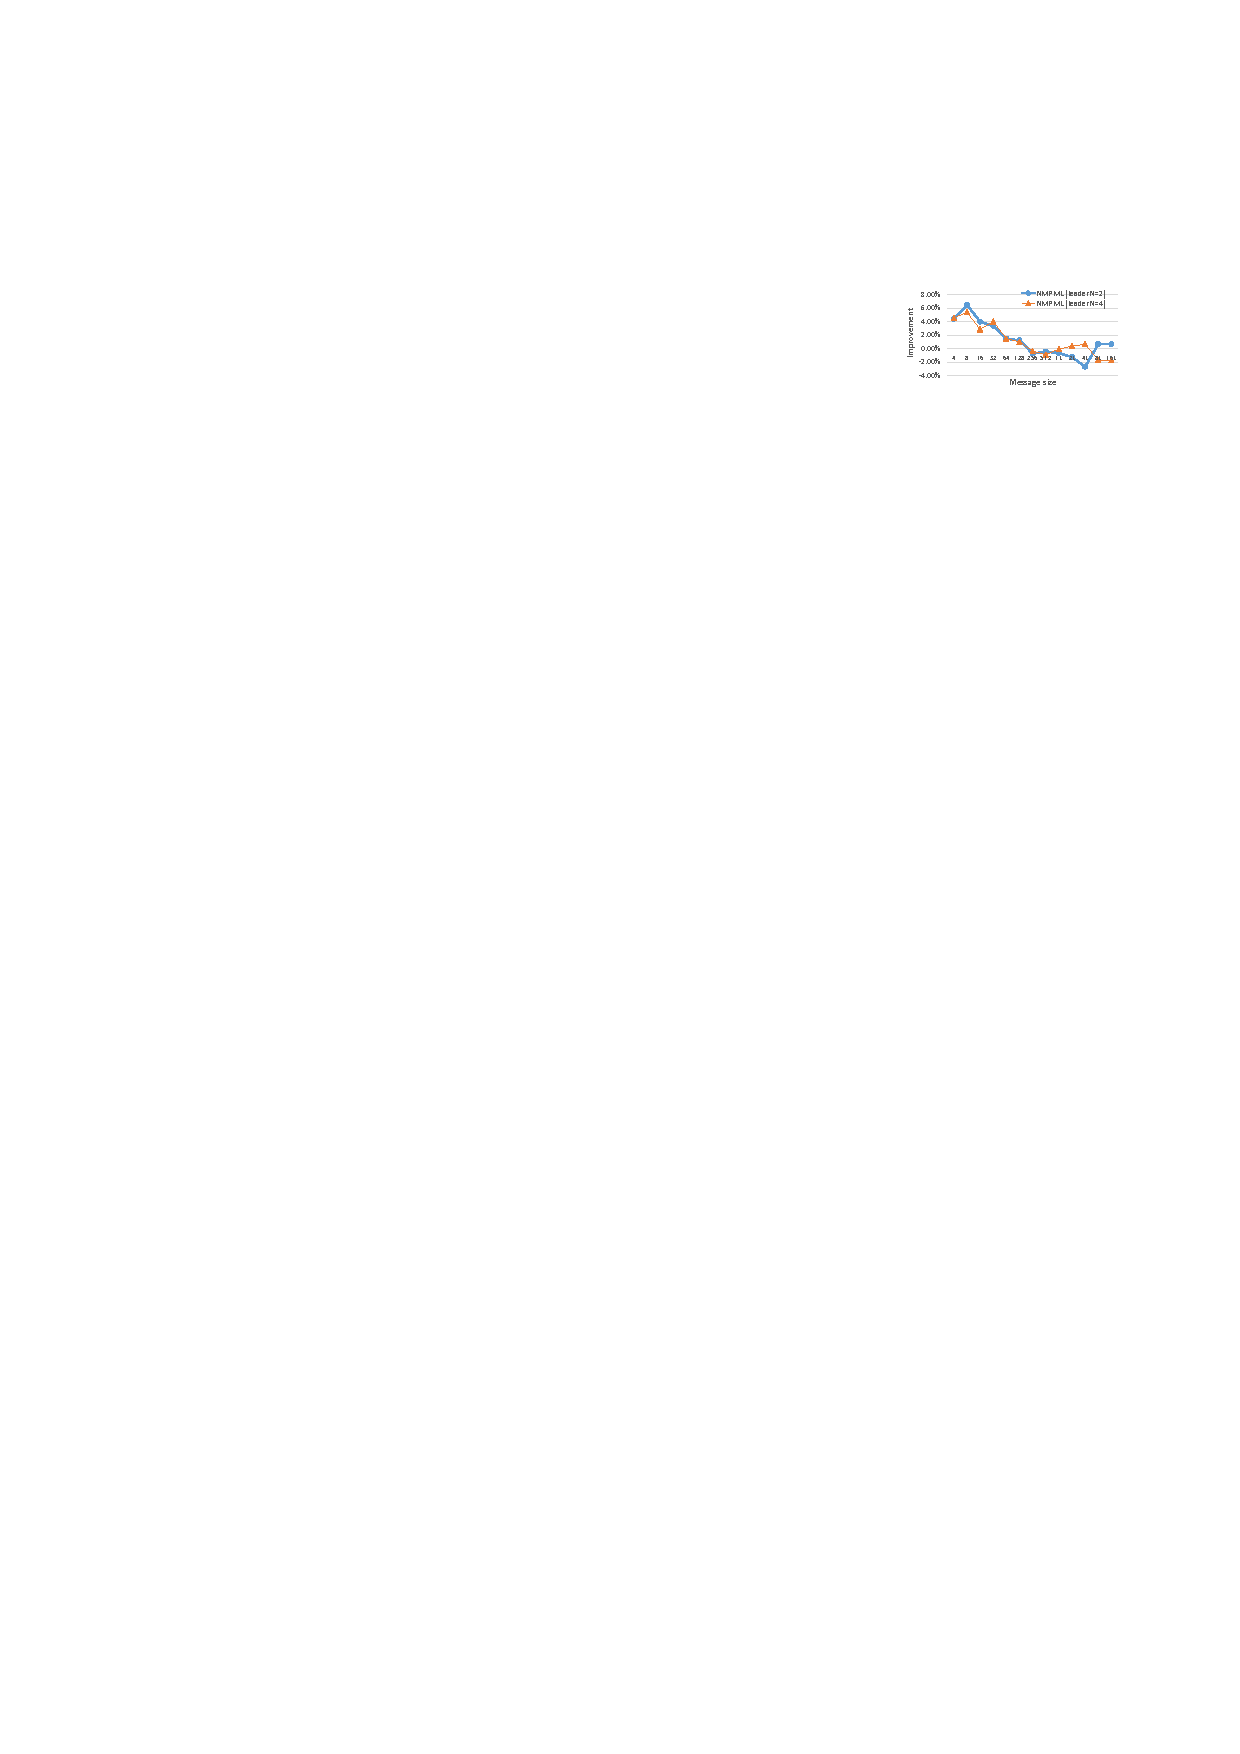
\includegraphics[width=0.45\textwidth]{./Figures/hpca/NMPML.pdf}}


    \subfigure[HPC-A:ONMPML compared to NMPML]{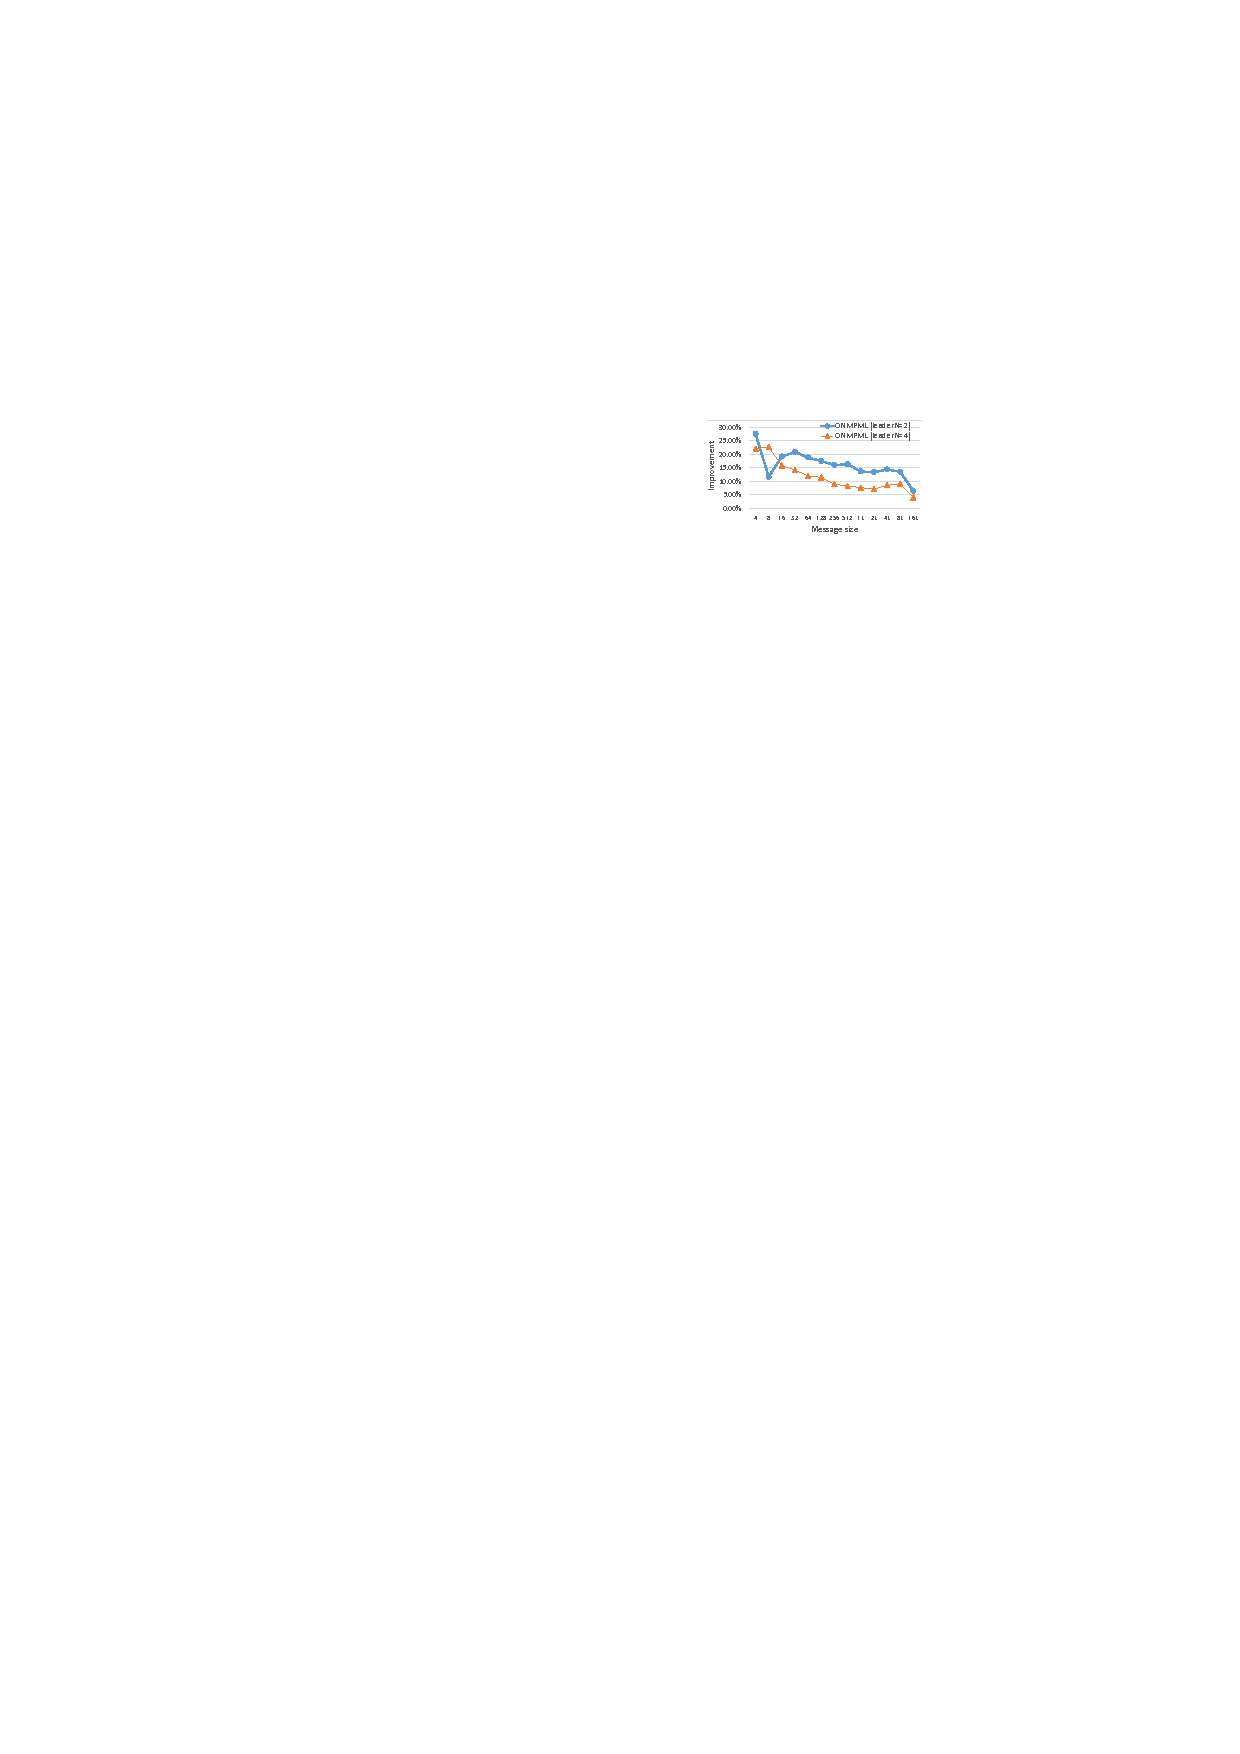
\includegraphics[width=0.45\textwidth]{./Figures/hpca/ONMPML.pdf}}
	\subfigure[HPC-A:ONMPML compared to MPI]{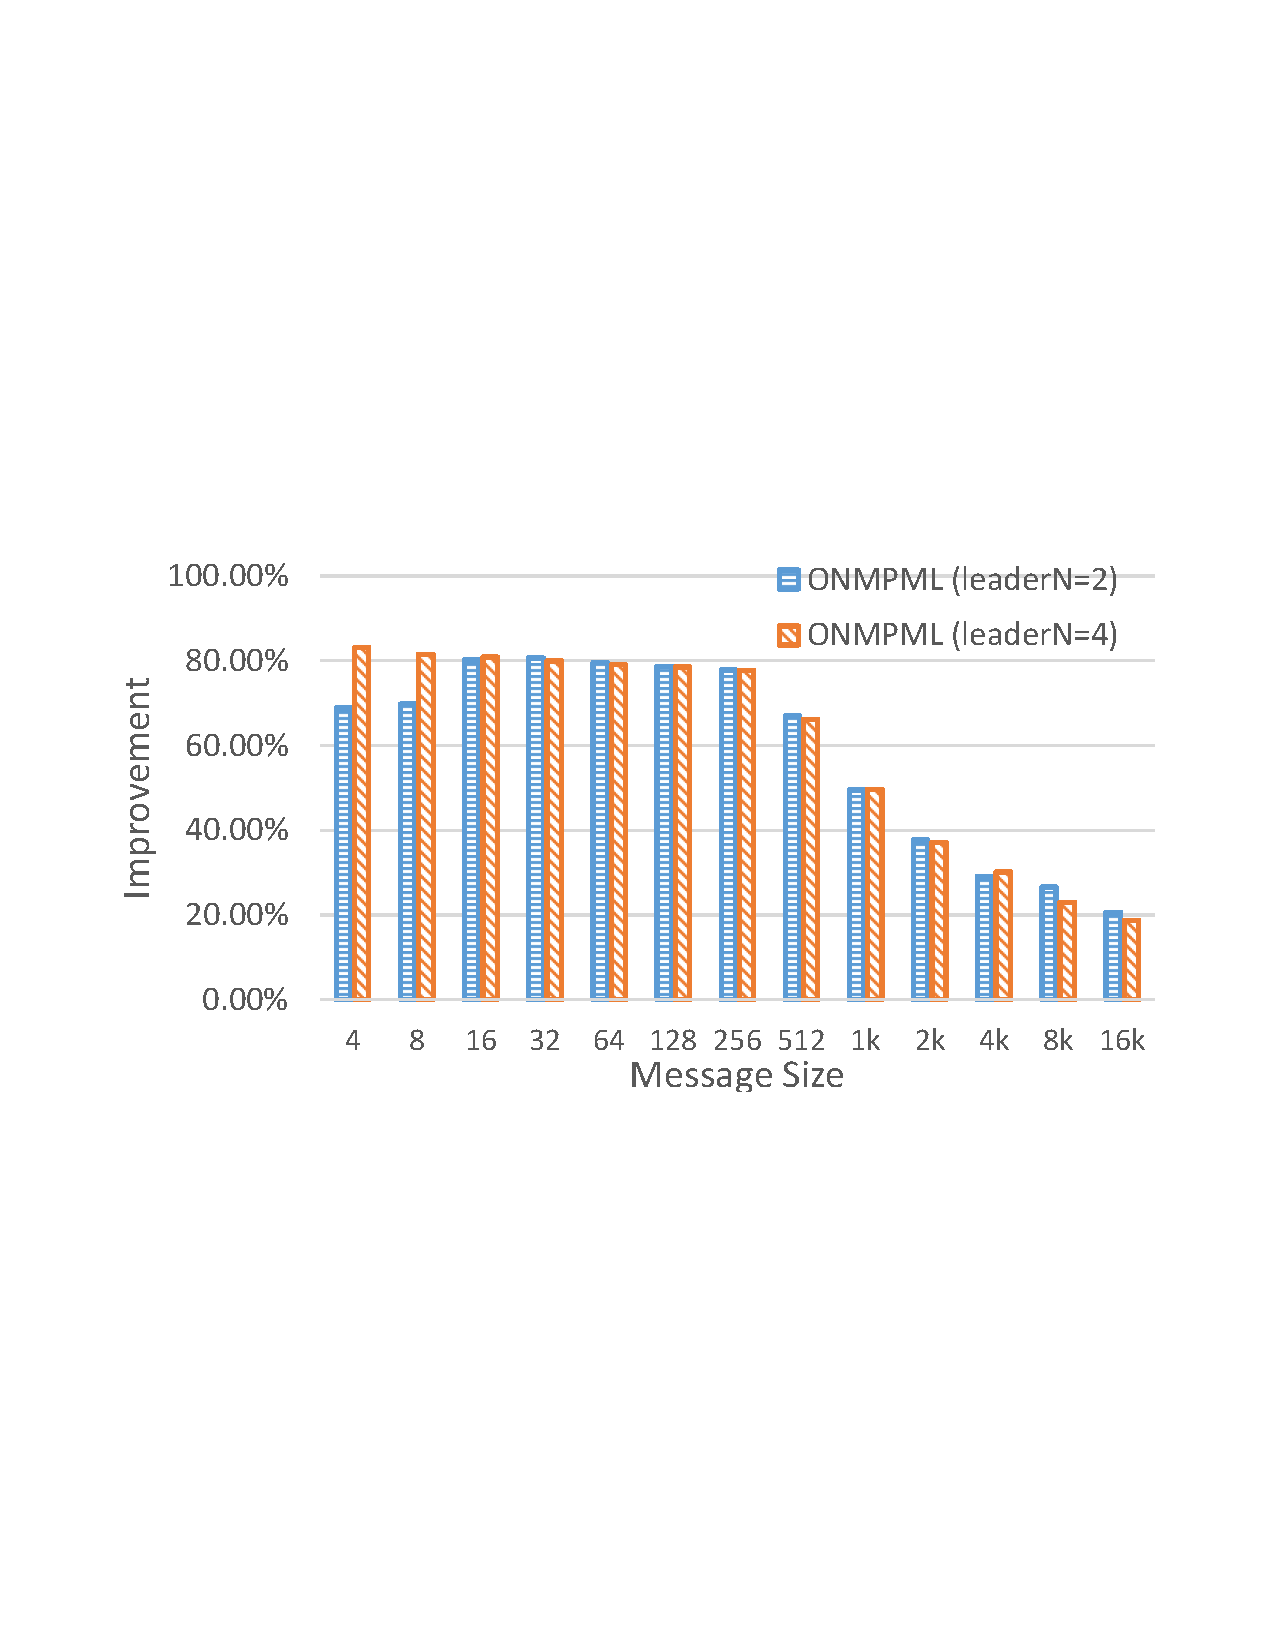
\includegraphics[width=0.45\textwidth]{./Figures/hpca/ONMPML-MPI.pdf}}
  \caption{Microbenchmark results of 256 nodes, 8192 processes alltoall collective on HPC-A.}
	\label{HPCA-EXPR}
	\vspace{0.2in}
\end{figure*}

\begin{algorithm}
\caption{all-to-all microbenchmark}\label{RDMASa2a}
{
	\For{ i in range(0,loopN)}
	{
		MPI\_Barrier(comm) \\
		startT = MPI\_Wtime() \\
		Alltoall() \\
		endT = MPI\_Wtime() \\
		totalT += (endT-start)
	}
	MPI\_Reduce(totalT,MaxT) \\
	MaxT $\leftarrow \frac{MaxT}{loopN}$ 
}
It compares the MPI\_Alltoall to our RDMA-based Alltoall (L-a2a, MPML, NMPML, ONMPML) on different HPC systems.
\end{algorithm}
\subsubsection{Microbenchmark Result on HPC-A}
The results of microbenchmark on four HPC systems are shown in Figure ~\ref{HPCA-EXPR}.
We can see that multi-endpoint, multi-leader alltoall (MPML) has a better performance than one leader alltoall (L-a2a).
When we using 4 leaders, its faster than 2 leader MPML.
In subfigure a of Figure \ref{HPCA-EXPR}, the improvement going down as the message getting larger.
As the HPC-A has the 1.3 GB/s bidirectional network bandwidth among these systems, which is far slower than the gatering/scattering bandwidth.
The whole alltoall is limited by the network bandwidth for large message.
As a result, MPML has a lesser performance improvement on a low-bandiwidth, large message alltoall.

Subfigure b of Figure \ref{HPCA-EXPR} show the performance of NUMA-aware MPML compared to MPML.
2-leader NMPML is compared to 2-leader MPML. 4-leader NMPML is the same the 2-leader NMPML.
For small message NUMA-aware MPML has a little performance improvement compared to MPML.
The large message has nearly no improvement.
This is same with the Figure \ref{UMA-aware-multi-leader}. The NUMA-aware gathering-scattering has batter throughput on small messages.

Subfigure c of Figure \ref{HPCA-EXPR} show that the ONMPML compared to corresponding NMPML.
ONMPML has a significant performance improvement. 
As ONMPML overlaped the inter-node and intra-node communication.
Subfigure d show the ONMPML compared to MPI\_Alltoall on HPC-A.
4-leader ONMPML has a 3.53x  speedup  on average compared to MPI\_Alltoall.
\subsubsection{Microbenchmark Result on HPC-B}
\begin{figure*}[!htb]
  \centering
    \subfigure[HPC-B:MPML compared to L-a2a]{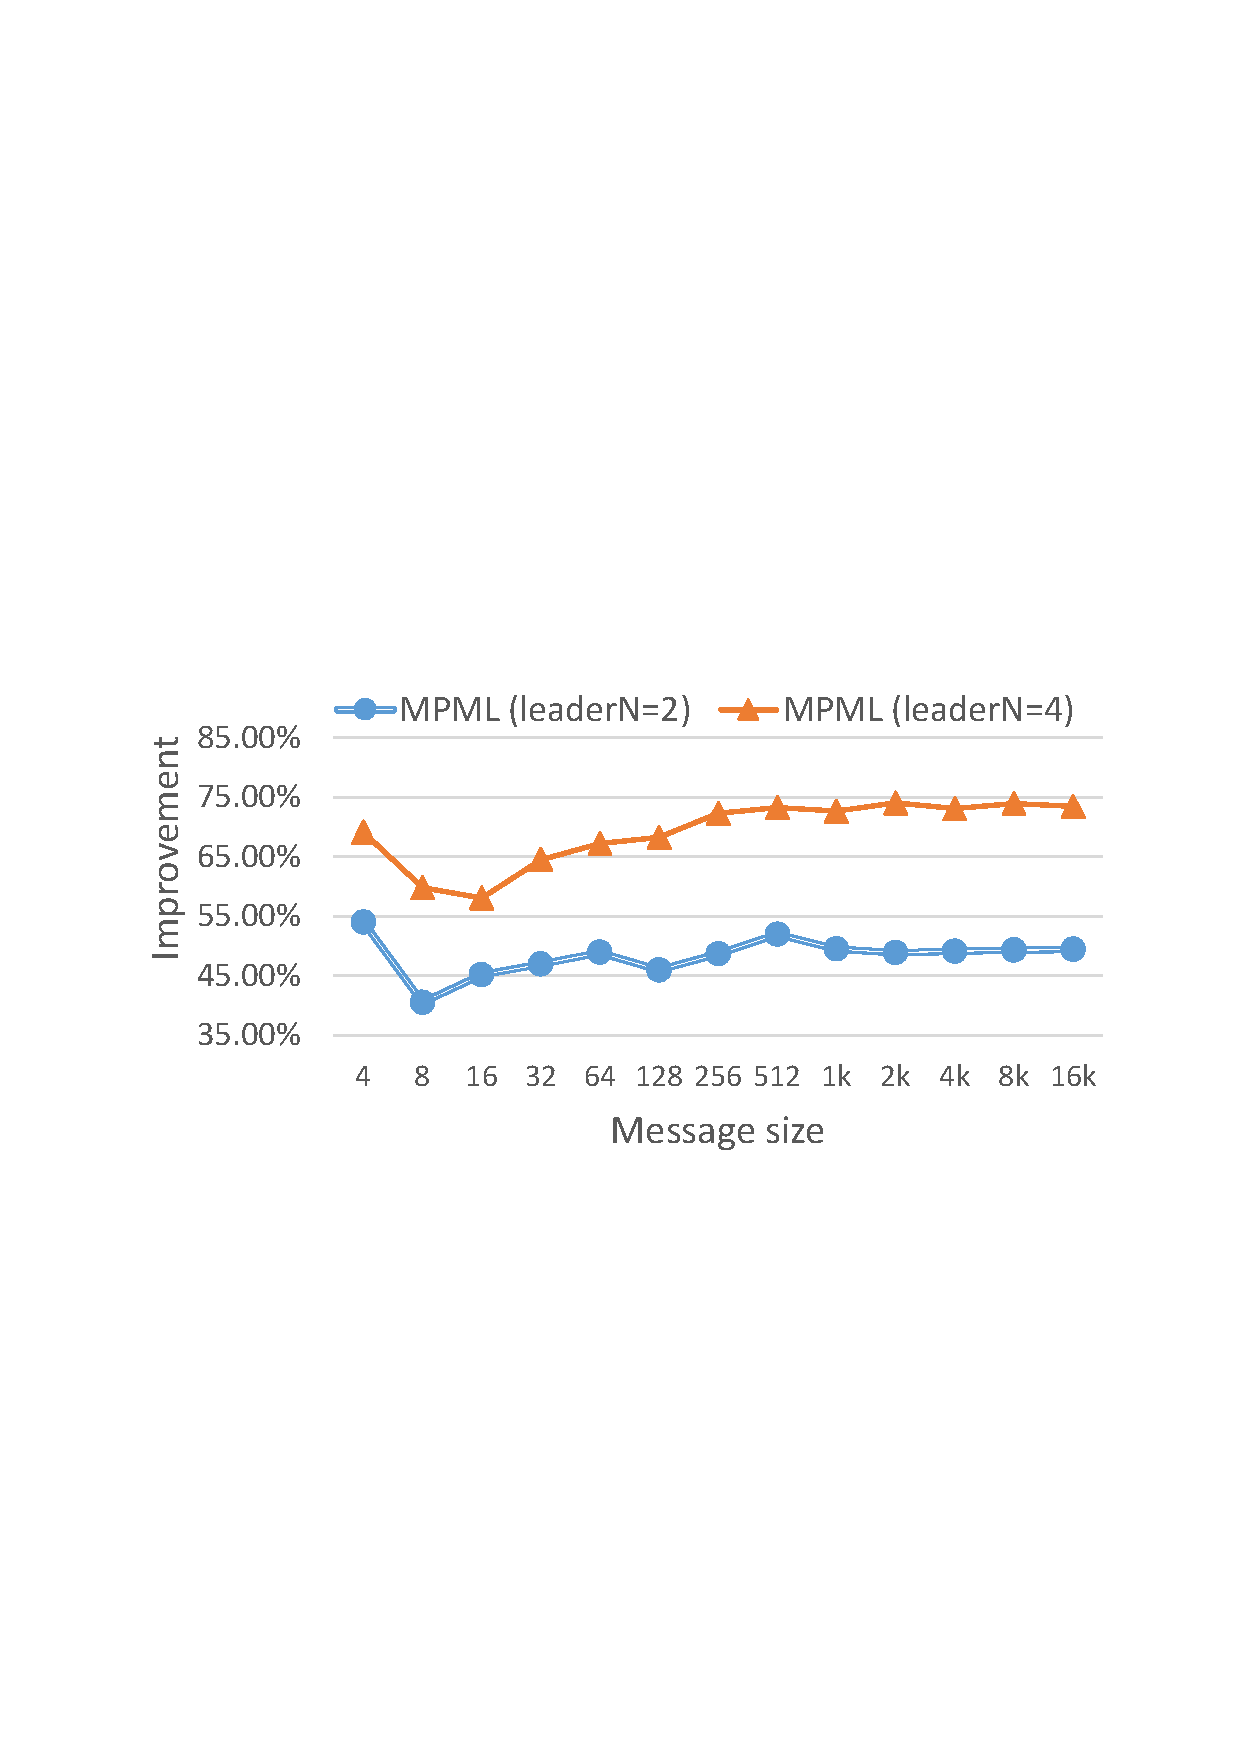
\includegraphics[width=0.45\textwidth]{./Figures/hpcd/MPML.pdf}}
	\subfigure[HPC-B:NMPML compared to MPML]{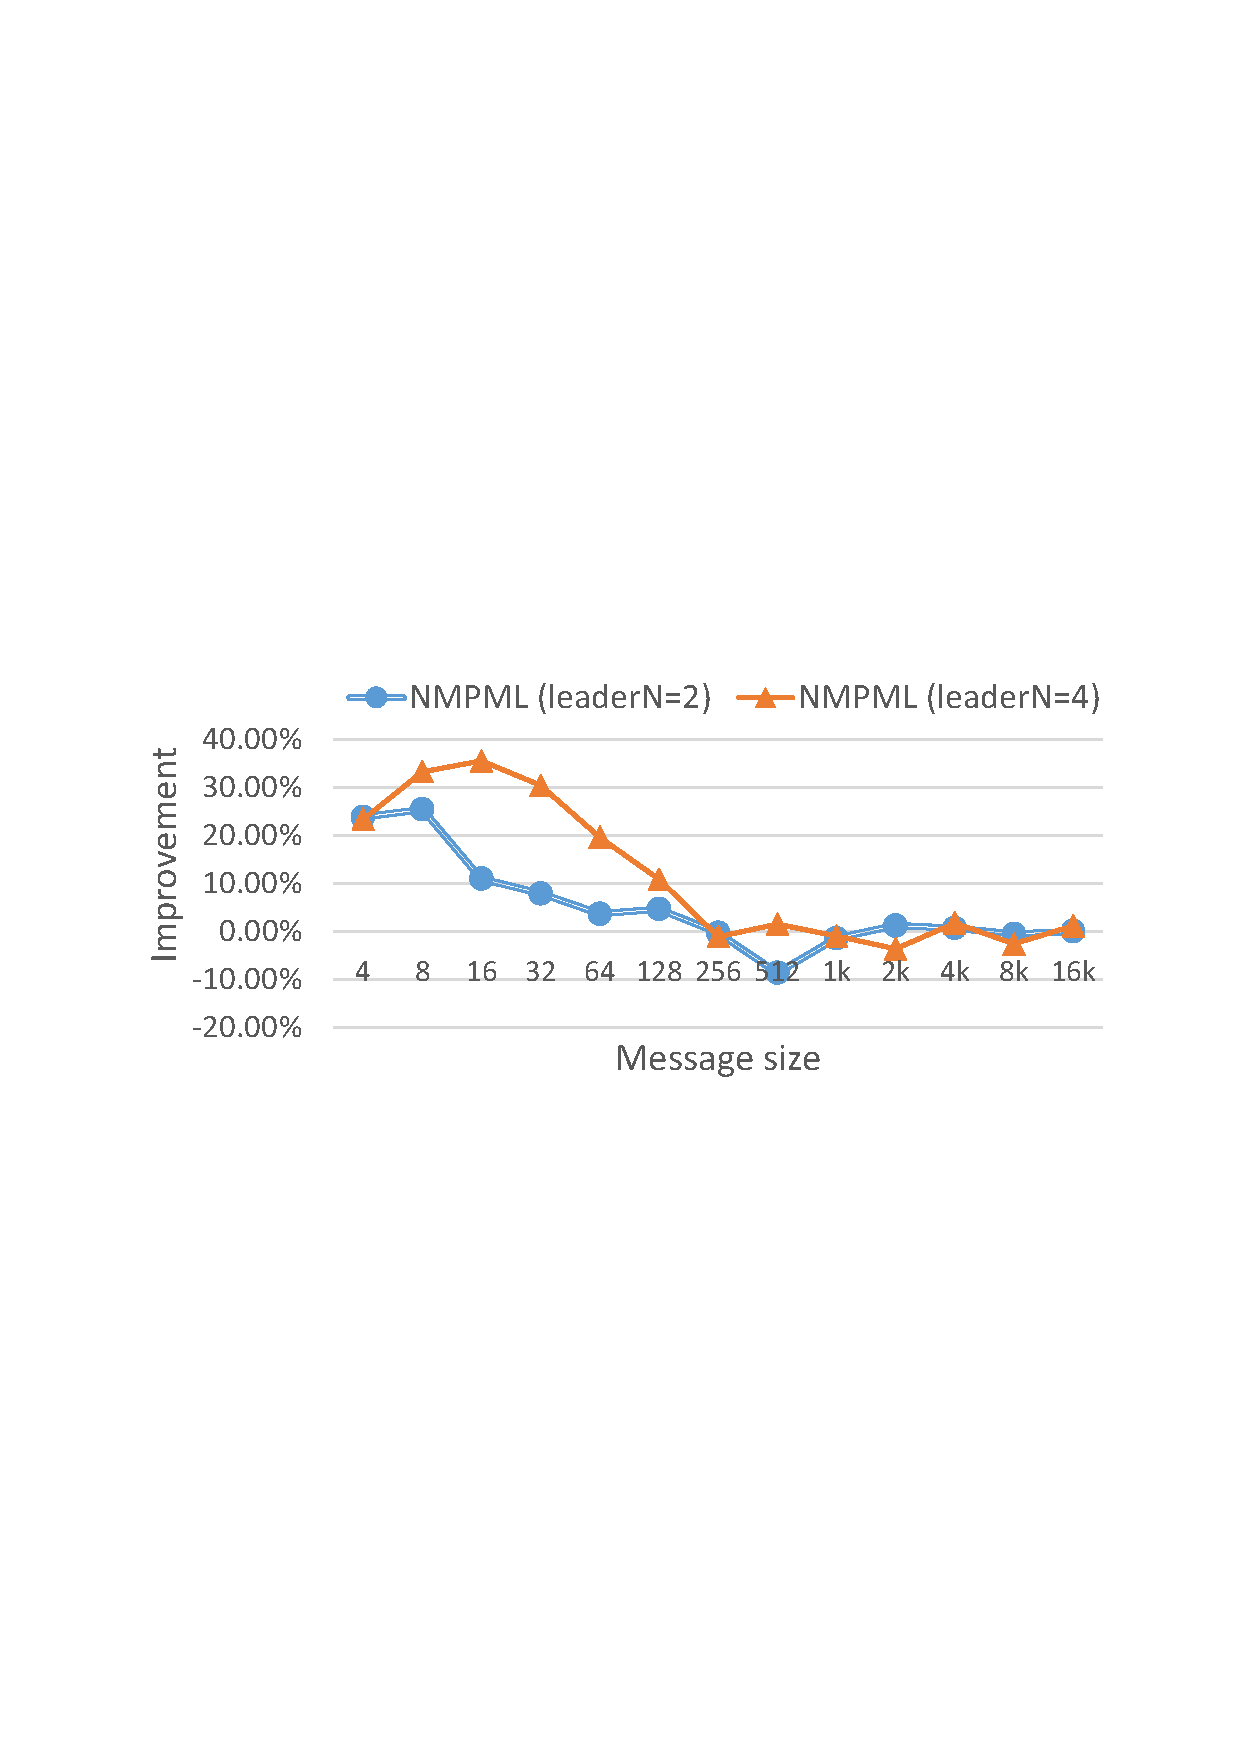
\includegraphics[width=0.45\textwidth]{./Figures/hpcd/NMPML.pdf}}


    \subfigure[HPC-B:ONMPML compared to NMPML]{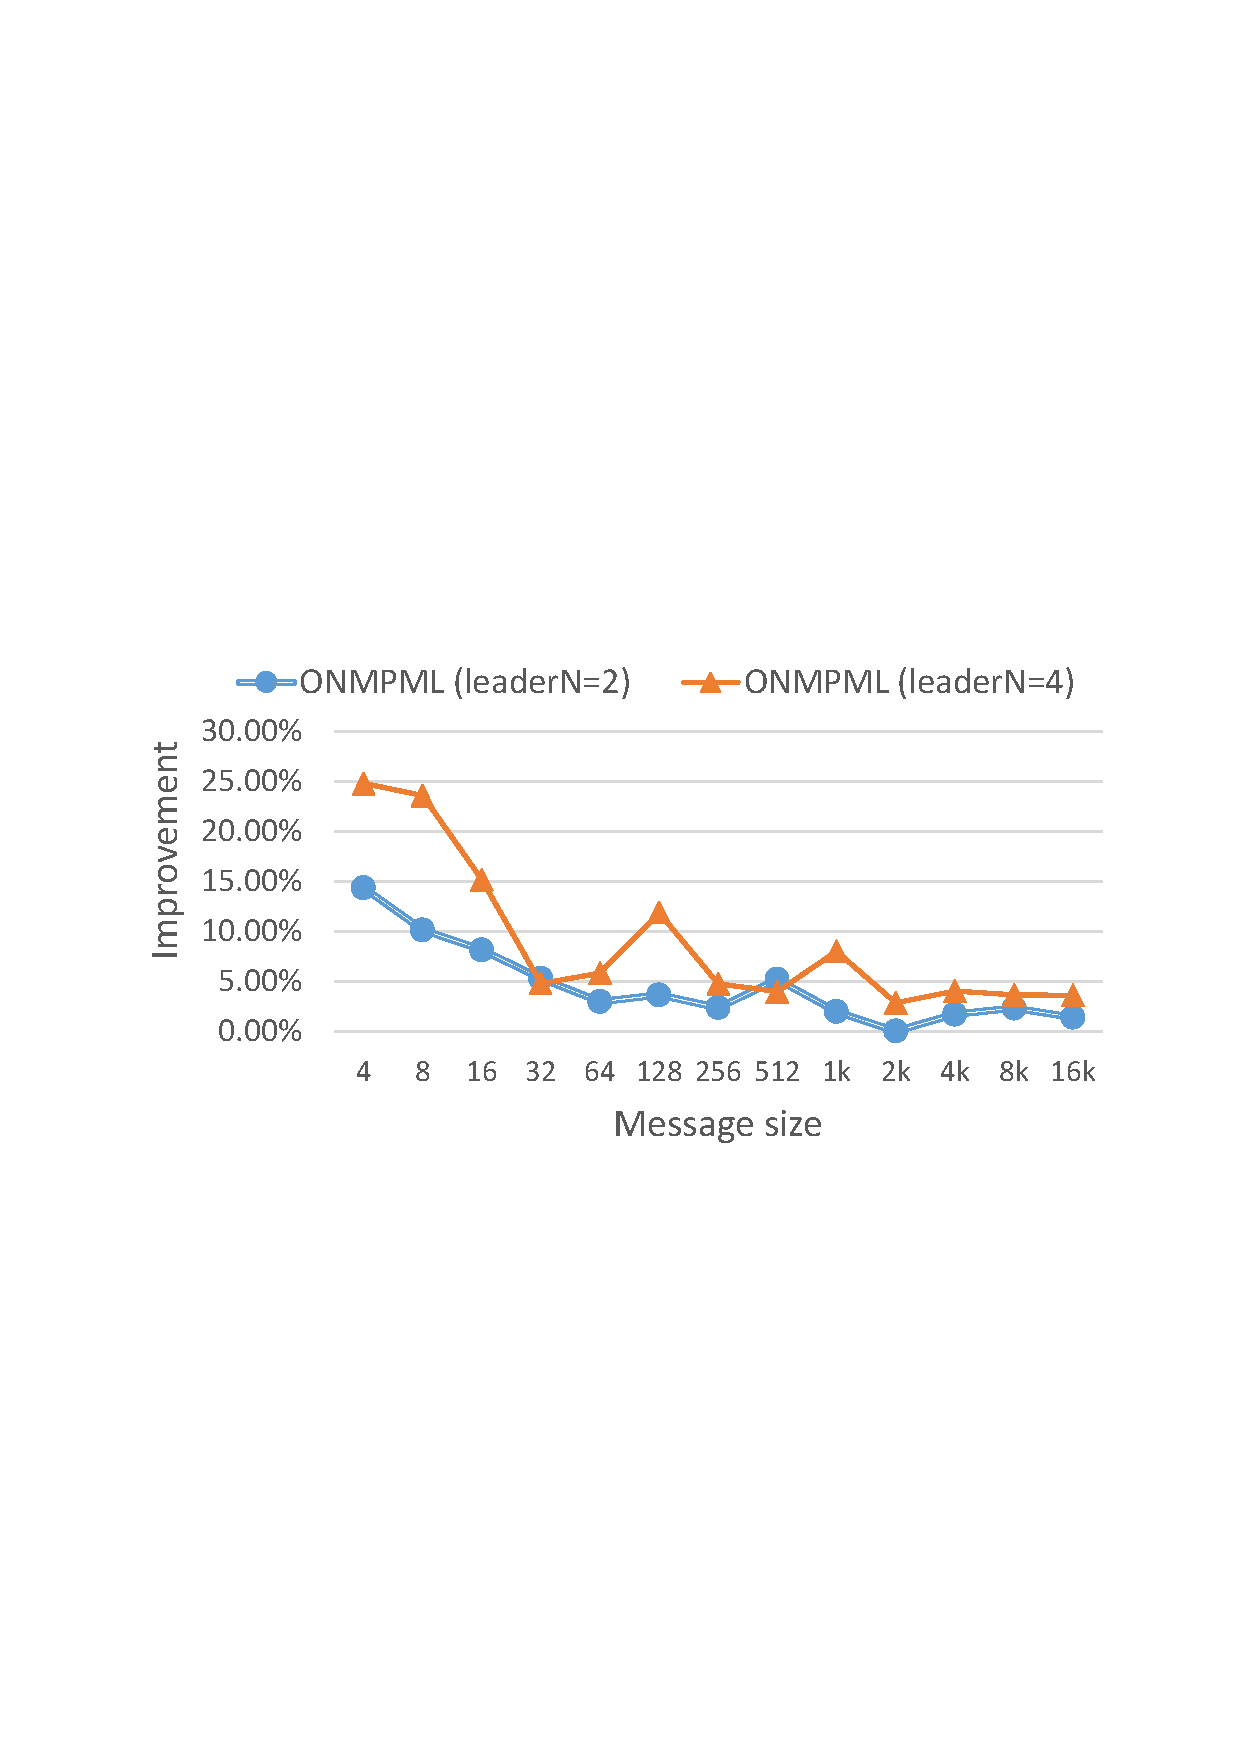
\includegraphics[width=0.45\textwidth]{./Figures/hpcd/ONMPML.pdf}}
	\subfigure[HPC-B:ONMPML compared to MPI]{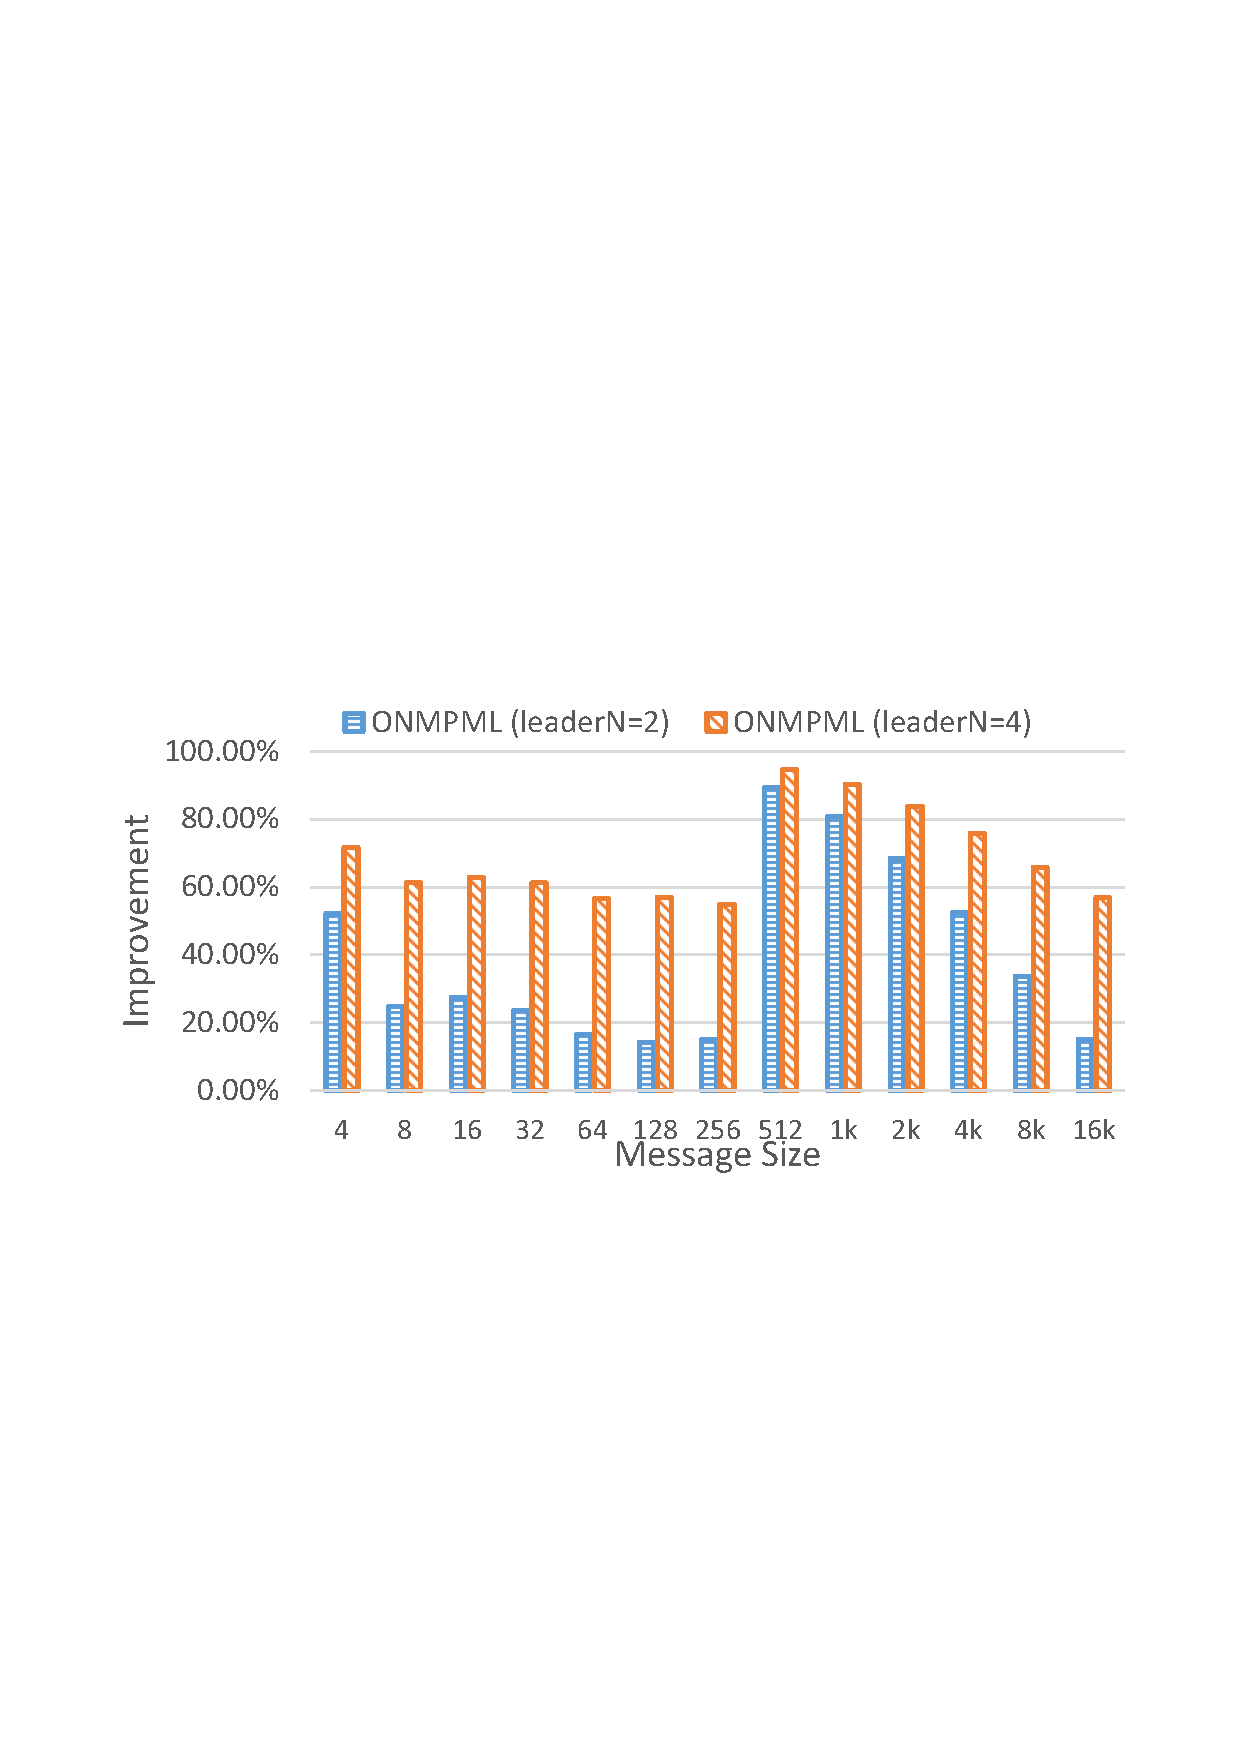
\includegraphics[width=0.45\textwidth]{./Figures/hpcd/ONMPML-MPI.pdf}}
  \caption{Microbenchmark results of 50 nodes, 1200 processes alltoall collective on HPC-B.}
	\label{HPCD-EXPR}
	\vspace{0.1in}
\end{figure*}
For subfigure a of Figure \ref{HPCD-EXPR}, MPML show a 45\% or 65\% improvement compared to L-a2a. This is because its bisectional network bandwidth is 11 GB/s. one leader's gathering/scattering throughput are 6 GB/s. The intra-node communication may take up a major part of communication overhead. As a result, MPML can obliviously improve the performance compare to L-a2a under the big messages.

For subfigure b of Figure \ref{HPCD-EXPR}, NMPML still show a little performance improvement for small messages.
Subfigure c show that 5\%(2-leader ONMPML) and 12.5\%(4-leader ONMPML) performance improvement compared to NMPML.
Compare to MPI\_Alltoall, 4-leader ONMPML acheives 3.7x speedup on average.

\subsection{HPCC-FFT Evaluation}
HPC Challenge is a benchmark suite which combines several benchmarks to test the performance of high-performance computer (HPC) systems \cite{luszczek2006hpc}.
Their is a global Fast Fourier Transforms (FFT) benchmark in HPCC.
FFT is very useful in applications such as spectral methods, signal processing and climate modeling.
HPCC global FFT doing a 1D FFT Z=FFT(X). 
MPI\_Alltoall is used to transpose matrix in global FFT.
We replace the MPI\_Alltoall with our 4-leader ONMPML based on GLEX RDMA (GLEX\_Alltoall).
We stested different vector size Ns. For HPC-A we test Ns=\{256,512,1024,2048\}.
For HPC-B, we test Ns=\{512,1024,2048,4096\}.
The result shown as Figure \~ref{App-EXPR}.
\begin{figure*}[!htb]
  \centering
    \subfigure[HPC-A: 256 nodes]{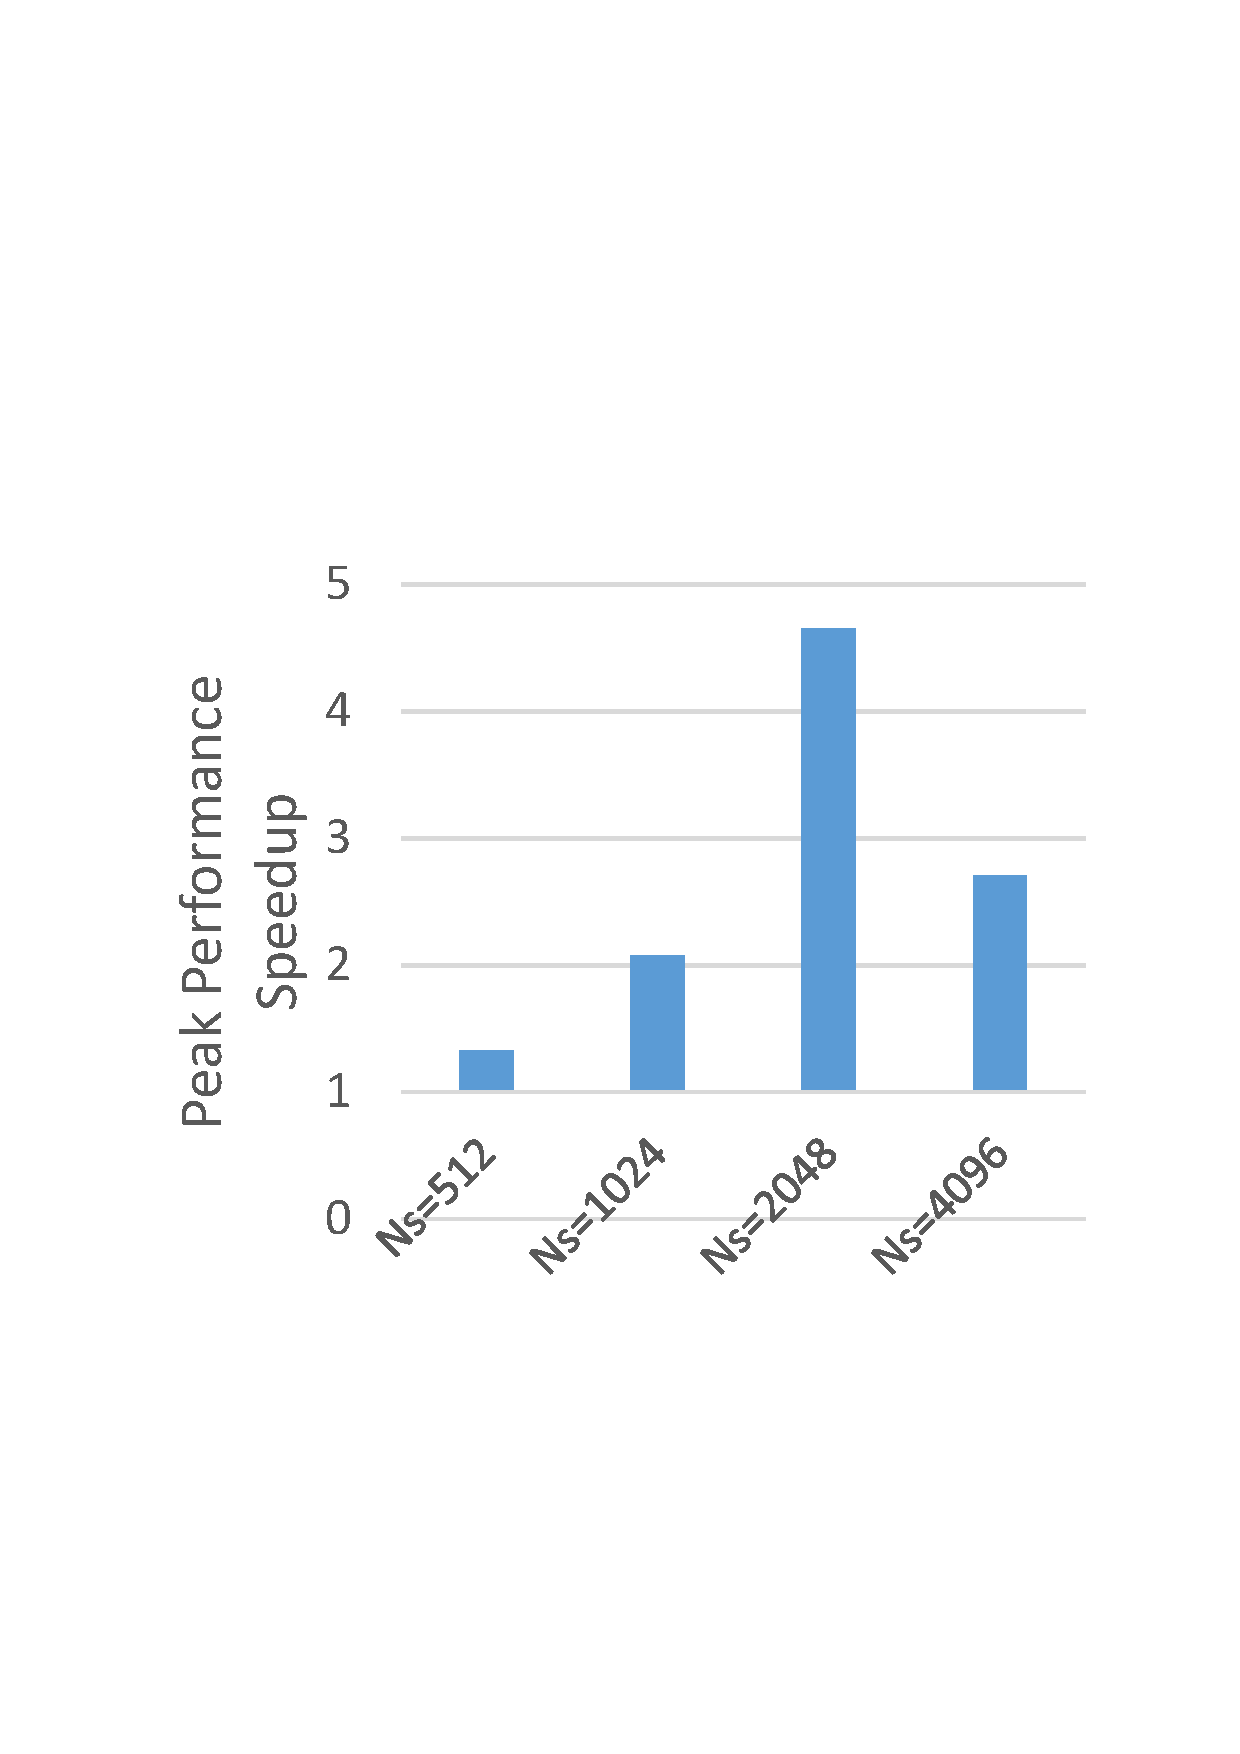
\includegraphics[width=0.32\textwidth]{./Figures/hpca/FFT.pdf}}
	\subfigure[HPC-B: 200 nodes]{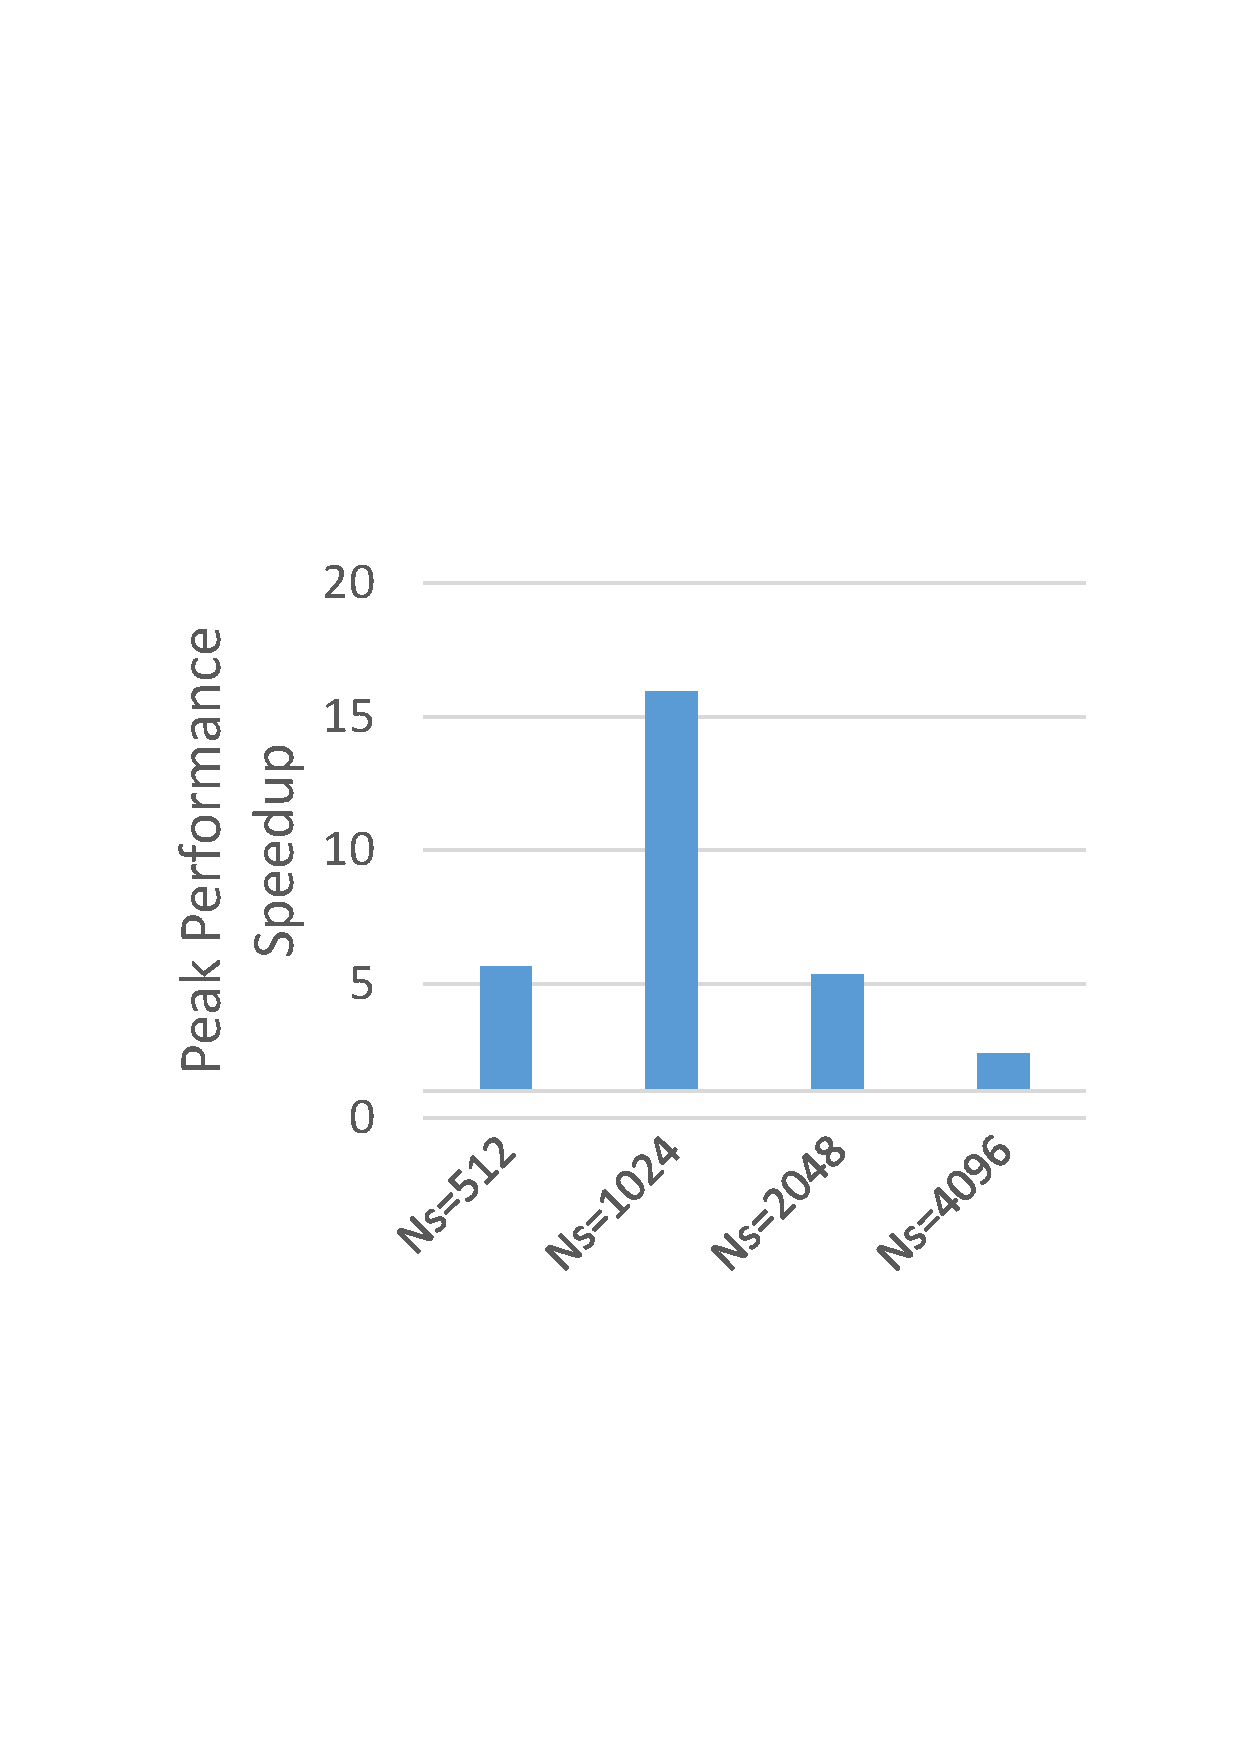
\includegraphics[width=0.32\textwidth]{./Figures/hpcd/FFT.pdf}}
  \caption{Application evaluations.}
	\label{App-EXPR}
	\vspace{0.1in}
\end{figure*}